% !TEX TS-program = pdflatex
% !TEX encoding = UTF-8 Unicode

% This file is a template using the "beamer" package to create slides for a talk or presentation
% - Giving a talk on some subject.
% - The talk is between 15min and 45min long.
% - Style is ornate.

% MODIFIED by Jonathan Kew, 2008-07-06
% The header comments and encoding in this file were modified for inclusion with TeXworks.
% The content is otherwise unchanged from the original distributed with the beamer package.

\documentclass{beamer}


% Copyright 2004 by Till Tantau <tantau@users.sourceforge.net>.
%
% In principle, this file can be redistributed and/or modified under
% the terms of the GNU Public License, version 2.
%
% However, this file is supposed to be a template to be modified
% for your own needs. For this reason, if you use this file as a
% template and not specifically distribute it as part of a another
% package/program, I grant the extra permission to freely copy and
% modify this file as you see fit and even to delete this copyright
% notice. 

\usepackage{multimedia}
\usepackage{tipa}

\mode<presentation>
{
  \usetheme{Warsaw}
  % or ...

  \setbeamercovered{transparent}
  % or whatever (possibly just delete it)
}


\usepackage[english]{babel}
% or whatever

\usepackage[utf8]{inputenc}
% or whatever

\usepackage{times}
\usepackage[T1]{fontenc}
% Or whatever. Note that the encoding and the font should match. If T1
% does not look nice, try deleting the line with the fontenc.


\title
{Attention and salience in lexically-guided perceptual learning}

\author
{Michael McAuliffe}
% - Use the \inst{?} command only if the authors have different
%   affiliation.

\institute
{}
% - Use the \inst command only if there are several affiliations.
% - Keep it simple, no one is interested in your street address.

\date
{2015 Research Report}

\subject{Talks}
% This is only inserted into the PDF information catalog. Can be left
% out. 



% If you have a file called "university-logo-filename.xxx", where xxx
% is a graphic format that can be processed by latex or pdflatex,
% resp., then you can add a logo as follows:

% \pgfdeclareimage[height=0.5cm]{university-logo}{university-logo-filename}
% \logo{\pgfuseimage{university-logo}}



% Delete this, if you do not want the table of contents to pop up at
% the beginning of each subsection:
\AtBeginSubsection[]
{
  \begin{frame}<beamer>{Outline}
    \tableofcontents[currentsection,currentsubsection]
  \end{frame}
}


% If you wish to uncover everything in a step-wise fashion, uncomment
% the following command: 

%\beamerdefaultoverlayspecification{<+->}


\begin{document}

\begin{frame}
  \titlepage
\end{frame}


\begin{frame}{Perceptual learning}
\movie{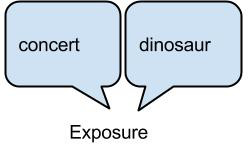
\includegraphics[width=0.45\textwidth]{pictures/exposure}}{audio/exposure.wav}
\hfill
\movie{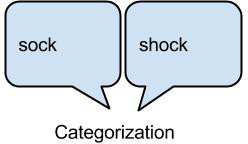
\includegraphics[width=0.45\textwidth]{pictures/categorization}}{audio/categorization.wav}

\vfill
\textbf{Research question:}

How do changes to a listener's attentional set in exposure affect perceptual learning in future categorization?
\vfill

\end{frame}

\begin{frame}{Attentional set}

Perception-oriented
\begin{itemize}
\item Phoneme-monitoring tasks
\item Discrimination of non-speech stimuli
\item Perceptual learning in psychophysics
\begin{itemize}
\item Perceptual learning effects don't generalize to new stimuli
\end{itemize}
\end{itemize}

Comprehension-oriented
\begin{itemize}
\item Word recognition tasks
\item Word identification tasks
\item Perceptual learning in speech perception
\begin{itemize}
\item Generalization to new items (and sometimes new speakers)
\end{itemize}
\end{itemize}

\vfill
\textbf{Hypothesis:}

Comprehension-oriented attentional sets allow for greater generalization than perception-oriented attentional sets.
\vfill

\end{frame}

\begin{frame}{Attentional set manipulation}

Explicit instructions
\begin{itemize}
\item "This speaker's 's' sounds are ambiguous'
\end{itemize}

Positional salience
\begin{itemize}
\item Sounds earlier in the word need to be perceived accurately
\item Sounds later in the word just need to confirm expectations from earlier sounds
\end{itemize}

Category typicality
\begin{itemize}
\item Productions that match a listeners expectations are less likely to be noticed
\item Productions that are unexpected for a category are more likely to be noticed
\end{itemize}

\end{frame}

\begin{frame}{Experiment 1}

\begin{minipage}{0.45\textwidth}
\textbf{Exposed to ambiguous /s/}
\begin{itemize}
\item 50\% between /s/ and /\textesh/
\end{itemize}

\textbf{Attention}
\begin{itemize}
\item No /s/-oriented instructions
\item Told /s/ would be ambiguous
\end{itemize}

\textbf{Position of /s/}
\begin{itemize}
\item \emph{Word initial}
\item Word medial
\end{itemize}
\end{minipage}
\hfill
\begin{minipage}{0.45\textwidth}
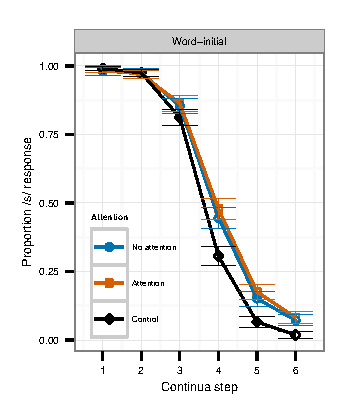
\includegraphics{graphs/exp1_categresults_present2-initial}
\end{minipage}

\end{frame}

\begin{frame}{Experiment 1}

\begin{minipage}{0.45\textwidth}
\textbf{Exposed to ambiguous /s/}
\begin{itemize}
\item 50\% between /s/ and /\textesh/
\end{itemize}

\textbf{Attention}
\begin{itemize}
\item No /s/-oriented instructions
\item Told /s/ would be ambiguous
\end{itemize}

\textbf{Position of /s/}
\begin{itemize}
\item Word initial
\item \emph{Word medial}
\end{itemize}
\end{minipage}
\hfill
\begin{minipage}{0.45\textwidth}
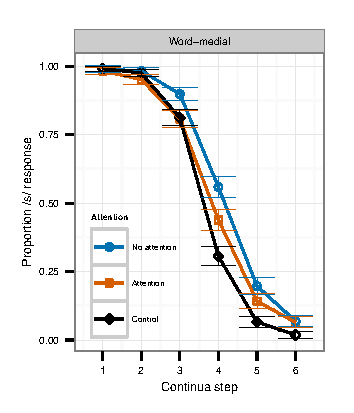
\includegraphics{graphs/exp1_categresults_present2-final}
\end{minipage}

\end{frame}

\begin{frame}{Experiment 2}

\begin{minipage}{0.45\textwidth}
\textbf{Exposed to ambiguous /s/}
\begin{itemize}
\item More like /\textesh/ than /s/
\end{itemize}

\textbf{Attention}
\begin{itemize}
\item No /s/-oriented instructions
\item Told /s/ would be ambiguous
\end{itemize}

\textbf{Position of /s/}
\begin{itemize}
\item \emph{Word initial}
\item Word medial
\end{itemize}
\end{minipage}
\hfill
\begin{minipage}{0.45\textwidth}
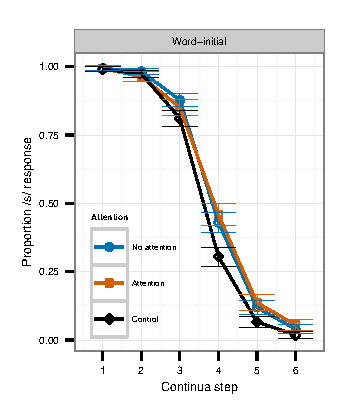
\includegraphics{graphs/exp2_categresults_present2-initial}
\end{minipage}

\end{frame}

\begin{frame}{Experiment 2}

\begin{minipage}{0.45\textwidth}
\textbf{Exposed to ambiguous /s/}
\begin{itemize}
\item More like /\textesh/ than /s/
\end{itemize}

\textbf{Attention}
\begin{itemize}
\item No /s/-oriented instructions
\item Told /s/ would be ambiguous
\end{itemize}

\textbf{Position of /s/}
\begin{itemize}
\item Word initial
\item \emph{Word medial}
\end{itemize}
\end{minipage}
\hfill
\begin{minipage}{0.45\textwidth}
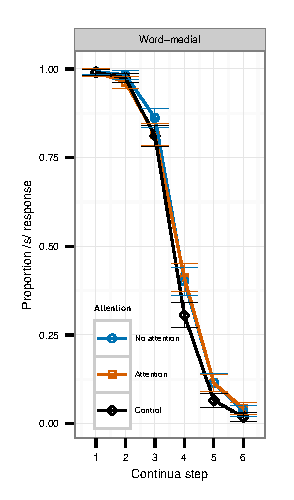
\includegraphics{graphs/exp2_categresults_present2-final}
\end{minipage}

\end{frame}

\begin{frame}{Summary}

\textbf{Comprehension-oriented}
\begin{itemize}
\item Default for the task
\item Most likely to be maintained when category atypicality and positional salience are low
\item Largest perceptual learning effects observed
\end{itemize}

\textbf{Perception-oriented}
\begin{itemize}
\item Perceptual learning effects are still present
\begin{itemize}
\item The exposure task as a whole was comprehension-oriented
\end{itemize}
\item Manipulations are not additive
\begin{itemize}
\item Equal amount of learning in the most salient, attended condition as in the others
\end{itemize}
\end{itemize}

\end{frame}


\end{document}


